\documentclass{article}
\usepackage[margin=1in]{geometry}
\usepackage{amsmath,amsthm,amssymb}
\usepackage{bbm,enumerate,mathtools}
\usepackage{tikz,pgfplots}
\usepackage{chessboard}
\usepackage[hidelinks]{hyperref}
\usepackage{multicol} % Problem 35

\newenvironment{question}{\begin{trivlist}\item[\textbf{Question.}]}{\end{trivlist}}
\newenvironment{note}{\begin{trivlist}\item[\textbf{Note.}]}{\end{trivlist}}
\newenvironment{references}{\begin{trivlist}\item[\textbf{References.}]}{\end{trivlist}}
\newenvironment{related}{\begin{trivlist}\item[\textbf{Related.}]\end{trivlist}\begin{enumerate}}{\end{enumerate}}


\begin{document}
\rating{3}{2}
My Twitter bot \href{https://twitter.com/oeisTriangles}{@oeisTriangles}
frequently tweets triangles based on OEIS sequences that appear to be
fractal-like. I asked about the triangle that comes from OEIS sequence A186759
on Math Stack Exchange, and got an
\href{https://math.stackexchange.com/a/4569833/121988}{answer from David Speyer}
that gives a theory of computing ``the fractal behavior of the coefficients of
rational generating functions modulo \(p\).''
\begin{figure}[ht!]
  \center
  
\includegraphics[trim={800 0 800 0}, clip, width=\textwidth/2]{assets/128_problem/triangle_fractal.jpg}
  \caption{
    The parity triangle based on the first 1024 rows of OEIS sequence A186759.
  }
\end{figure}

\begin{figure}[ht!]
\noindent
% 
\includegraphics[trim={800 0 800 0}, clip, width=4cm]{assets/128_problem/A026747_2022-08-14.png}
% 
\includegraphics[trim={800 0 800 0}, clip, width=4cm]{assets/128_problem/A053538_2021-07-23.png}
% 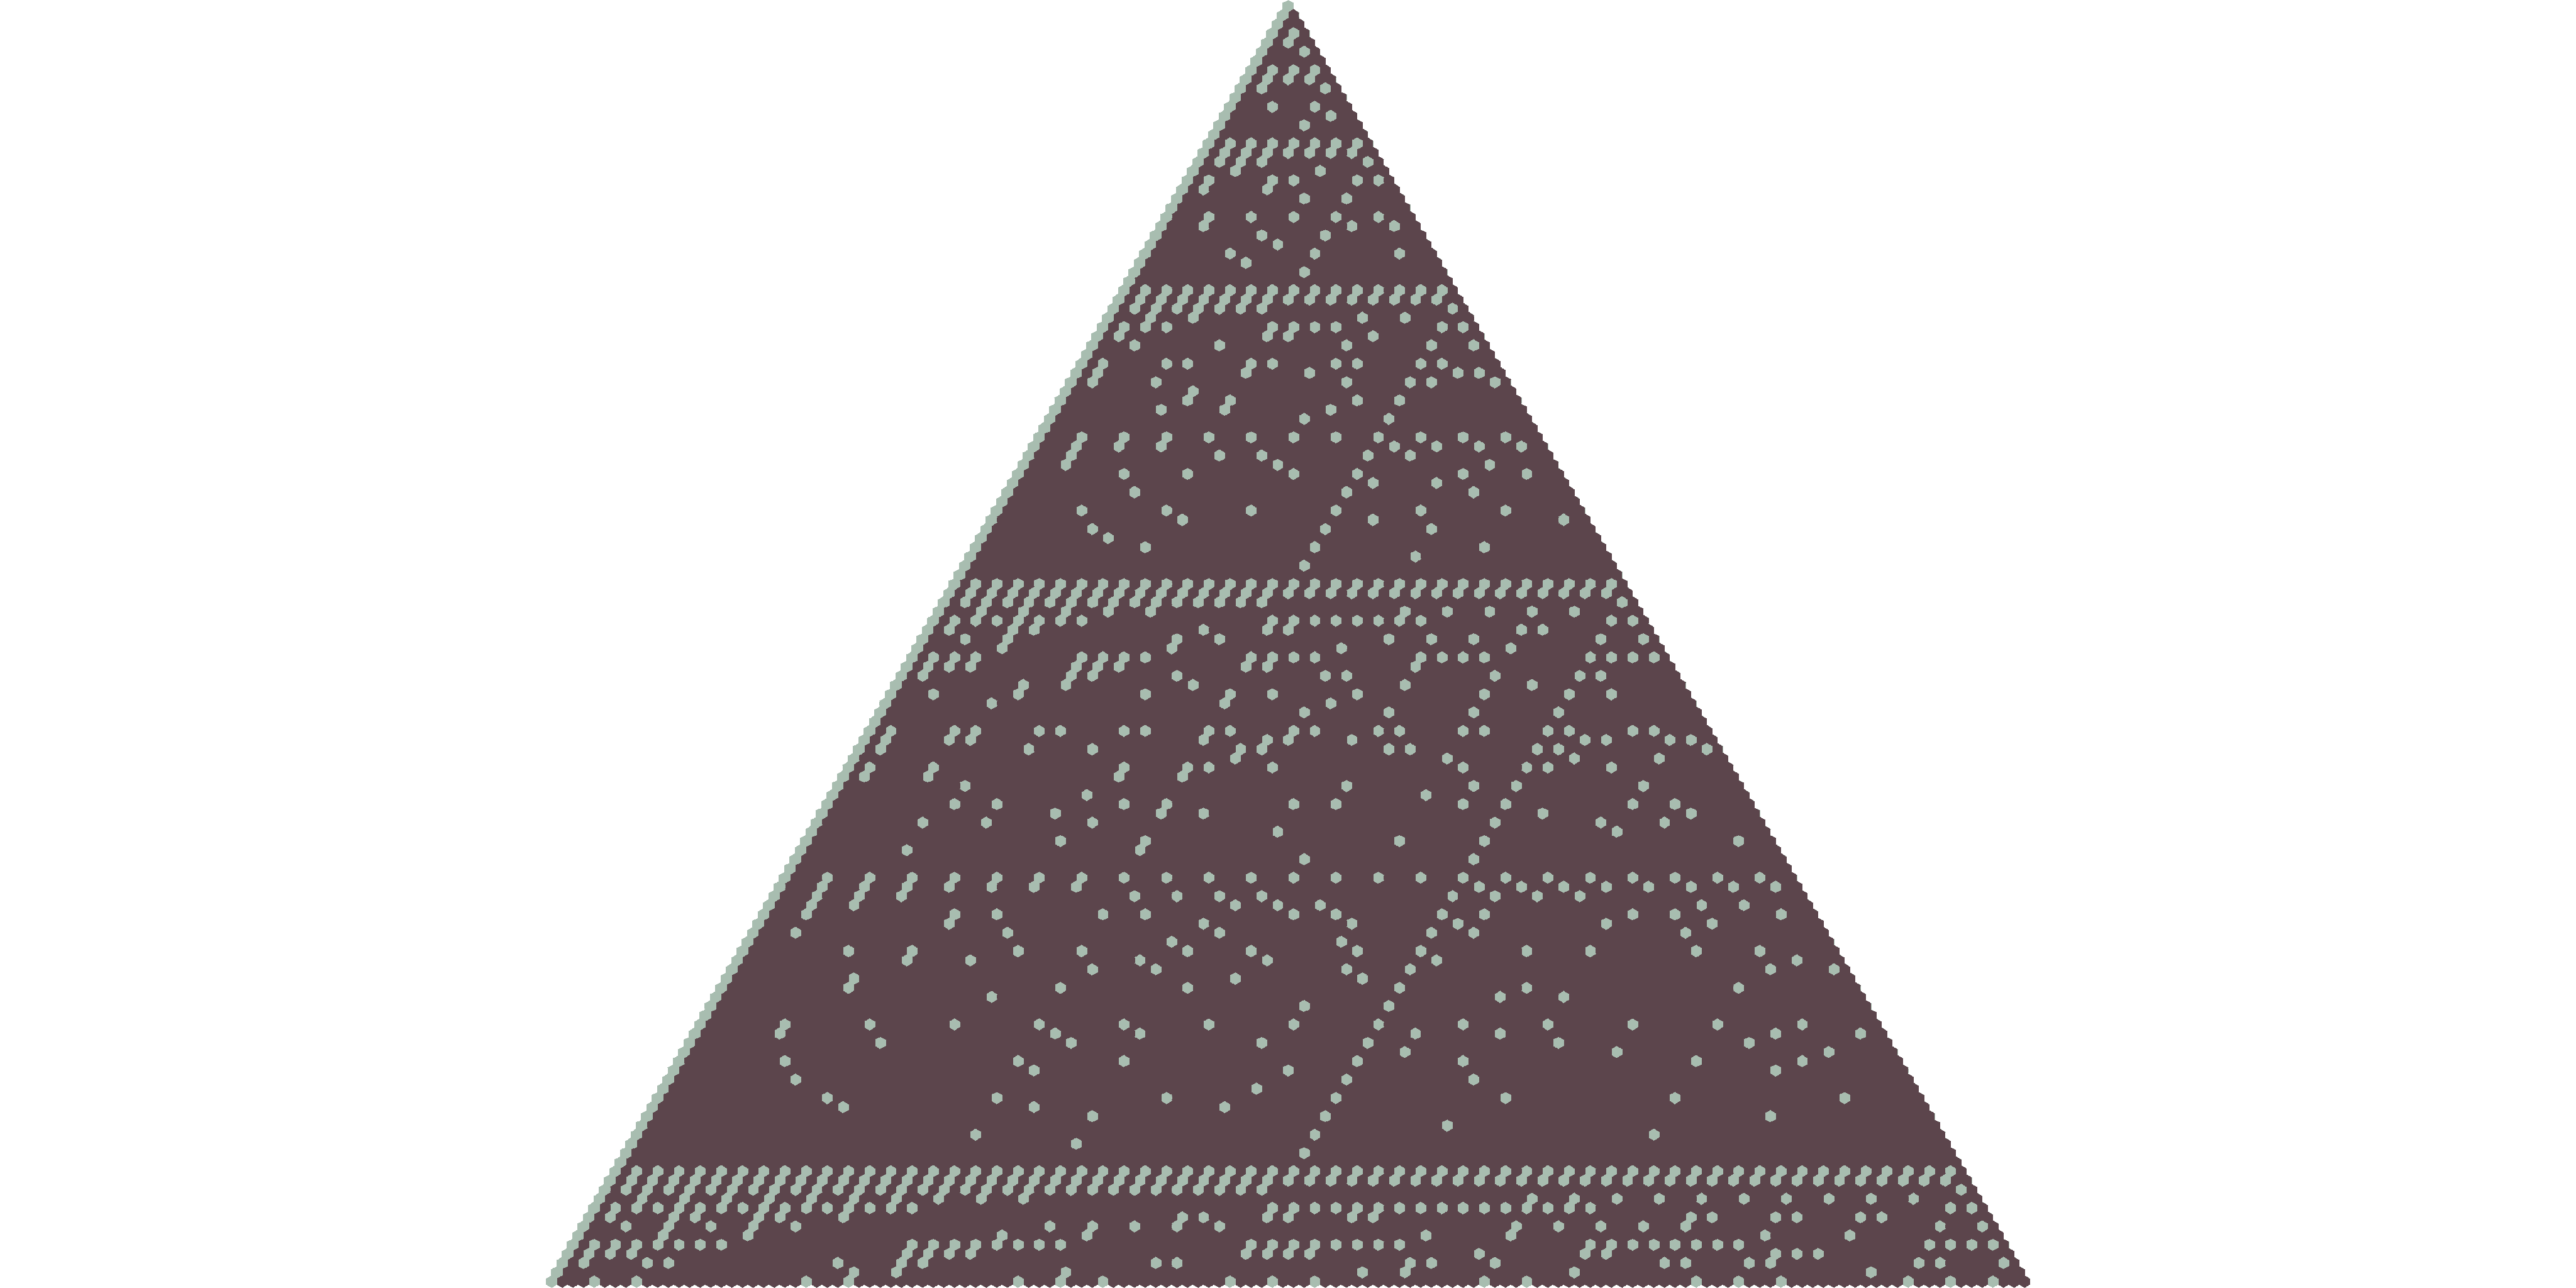
\includegraphics[trim={800 0 800 0}, clip, width=4cm]{assets/128_problem/A096130_2022-08-19.png}
% 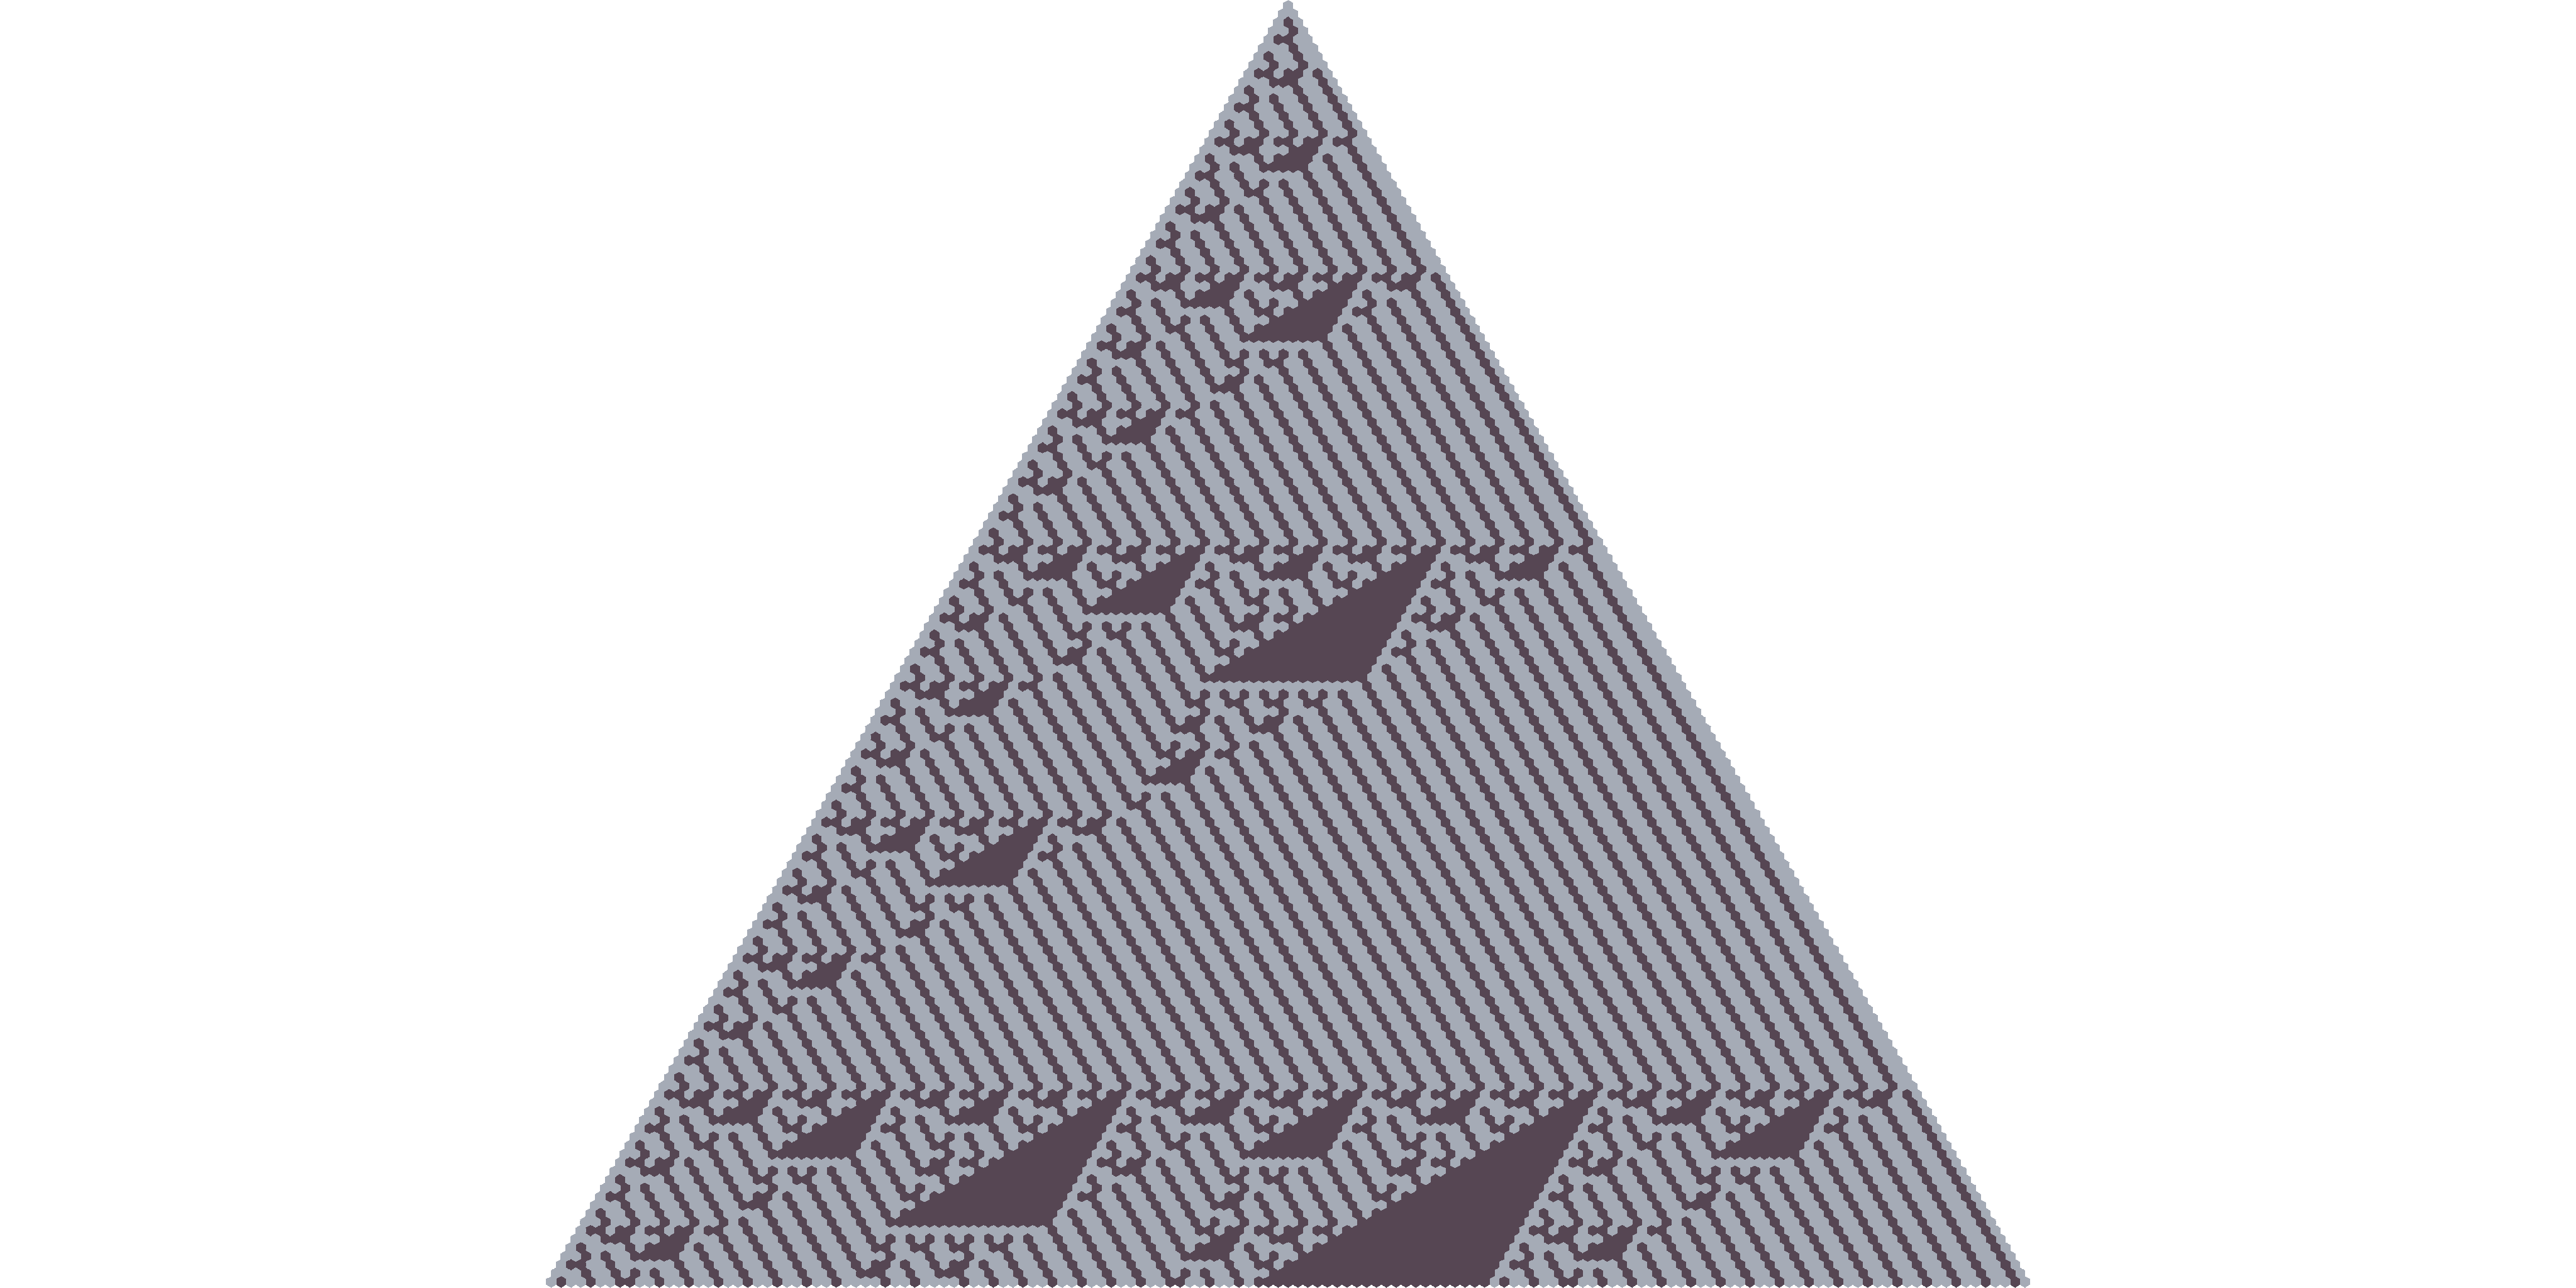
\includegraphics[trim={800 0 800 0}, clip, width=4cm]{assets/128_problem/A096465_2022_02-03.png}
% 
\includegraphics[trim={800 0 800 0}, clip, width=4cm]{assets/128_problem/A102661_2022-07-18.png}
% 
\includegraphics[trim={800 0 800 0}, clip, width=4cm]{assets/128_problem/A105422_2022-01-26.png}
% 
\includegraphics[trim={800 0 800 0}, clip, width=4cm]{assets/128_problem/A105599_2022-09-25.png}
% 
\includegraphics[trim={800 0 800 0}, clip, width=4cm]{assets/128_problem/A108947_2021-08-22.png}
% 
\includegraphics[trim={800 0 800 0}, clip, width=4cm]{assets/128_problem/A118354_2022-05-13.png}
% 
\includegraphics[trim={800 0 800 0}, clip, width=4cm]{assets/128_problem/A118964_2022-06-18.png}
% 
\includegraphics[trim={800 0 800 0}, clip, width=4cm]{assets/128_problem/A136431_2022-08-11.png}
% 
\includegraphics[trim={800 0 800 0}, clip, width=4cm]{assets/128_problem/A143565_2022-02-02.png}
% 
\includegraphics[trim={800 0 800 0}, clip, width=4cm]{assets/128_problem/A145152_2022-09-14.png}
% 
\includegraphics[trim={800 0 800 0}, clip, width=4cm]{assets/128_problem/A154844_2021-05-07.png}
% 
\includegraphics[trim={800 0 800 0}, clip, width=4cm]{assets/128_problem/A156003_2022_07-01.png}
% 
\includegraphics[trim={800 0 800 0}, clip, width=4cm]{assets/128_problem/A176082_2022-01-21.png}
% 
\includegraphics[trim={800 0 800 0}, clip, width=4cm]{assets/128_problem/A176124_2022-08-17.png}
% 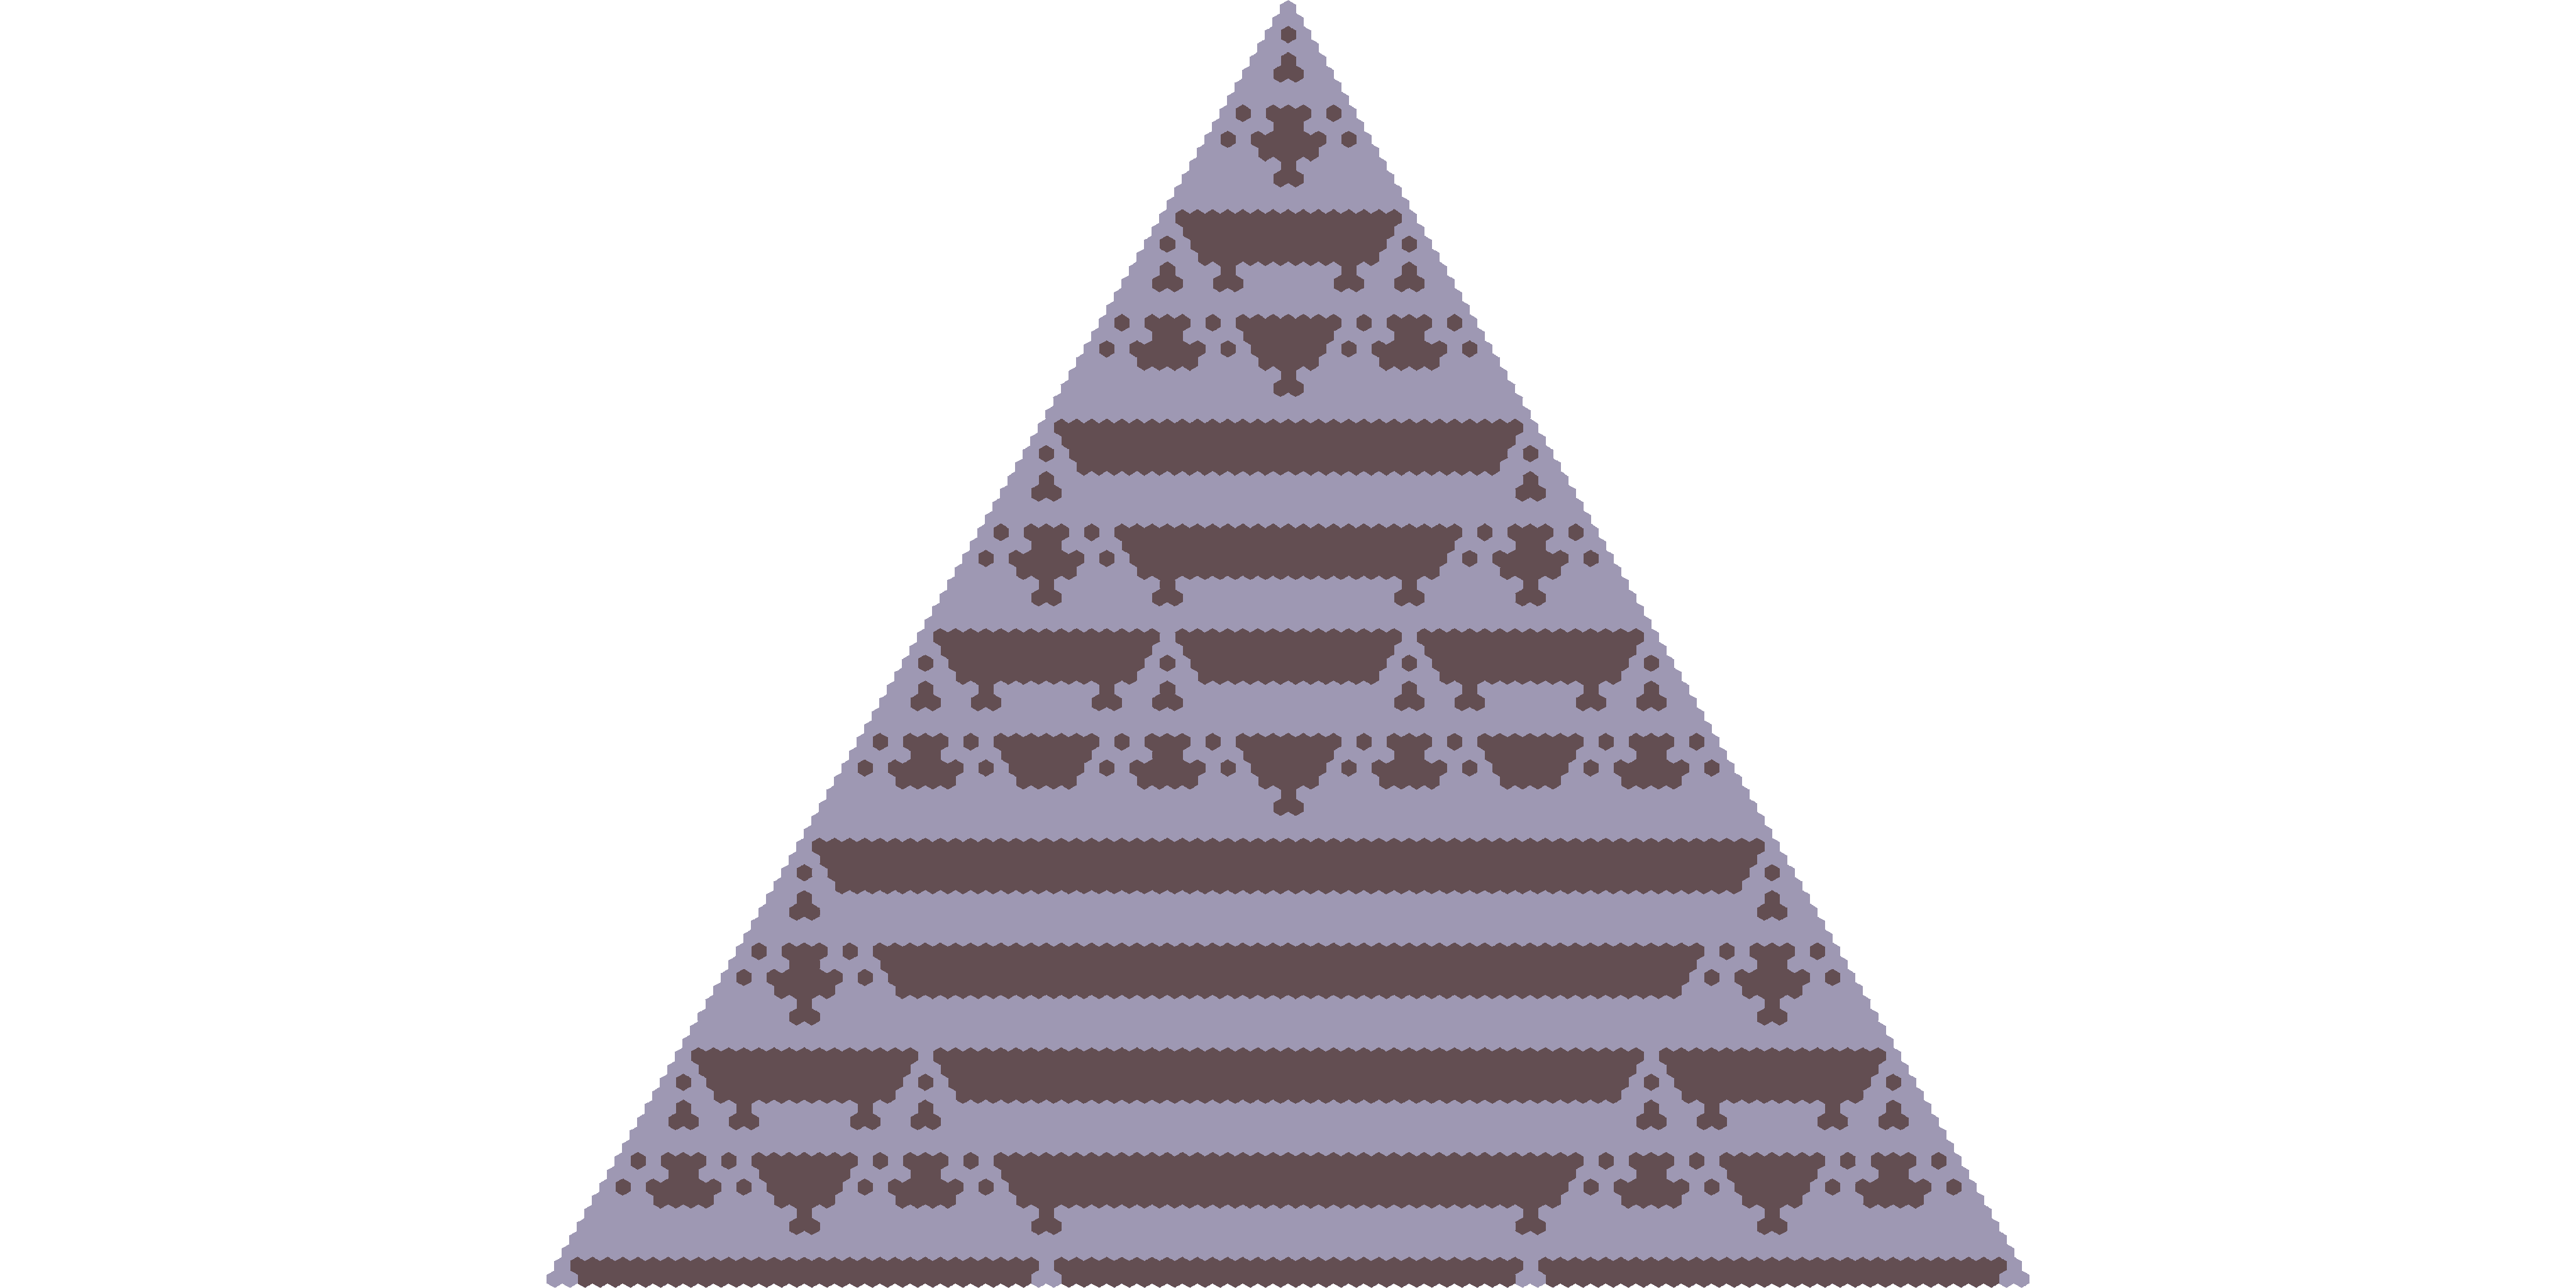
\includegraphics[trim={800 0 800 0}, clip, width=4cm]{assets/128_problem/A176125_2022-01-31.png}
% 
\includegraphics[trim={800 0 800 0}, clip, width=4cm]{assets/128_problem/A176331_2022-02-09.png}
% 
\includegraphics[trim={800 0 800 0}, clip, width=4cm]{assets/128_problem/A180177_2021-11-02.png}
% 
\includegraphics[trim={800 0 800 0}, clip, width=4cm]{assets/128_problem/A215861_2022-02-17.png}
% 
\includegraphics[trim={800 0 800 0}, clip, width=4cm]{assets/128_problem/A229223_2021-05-06.png}
% 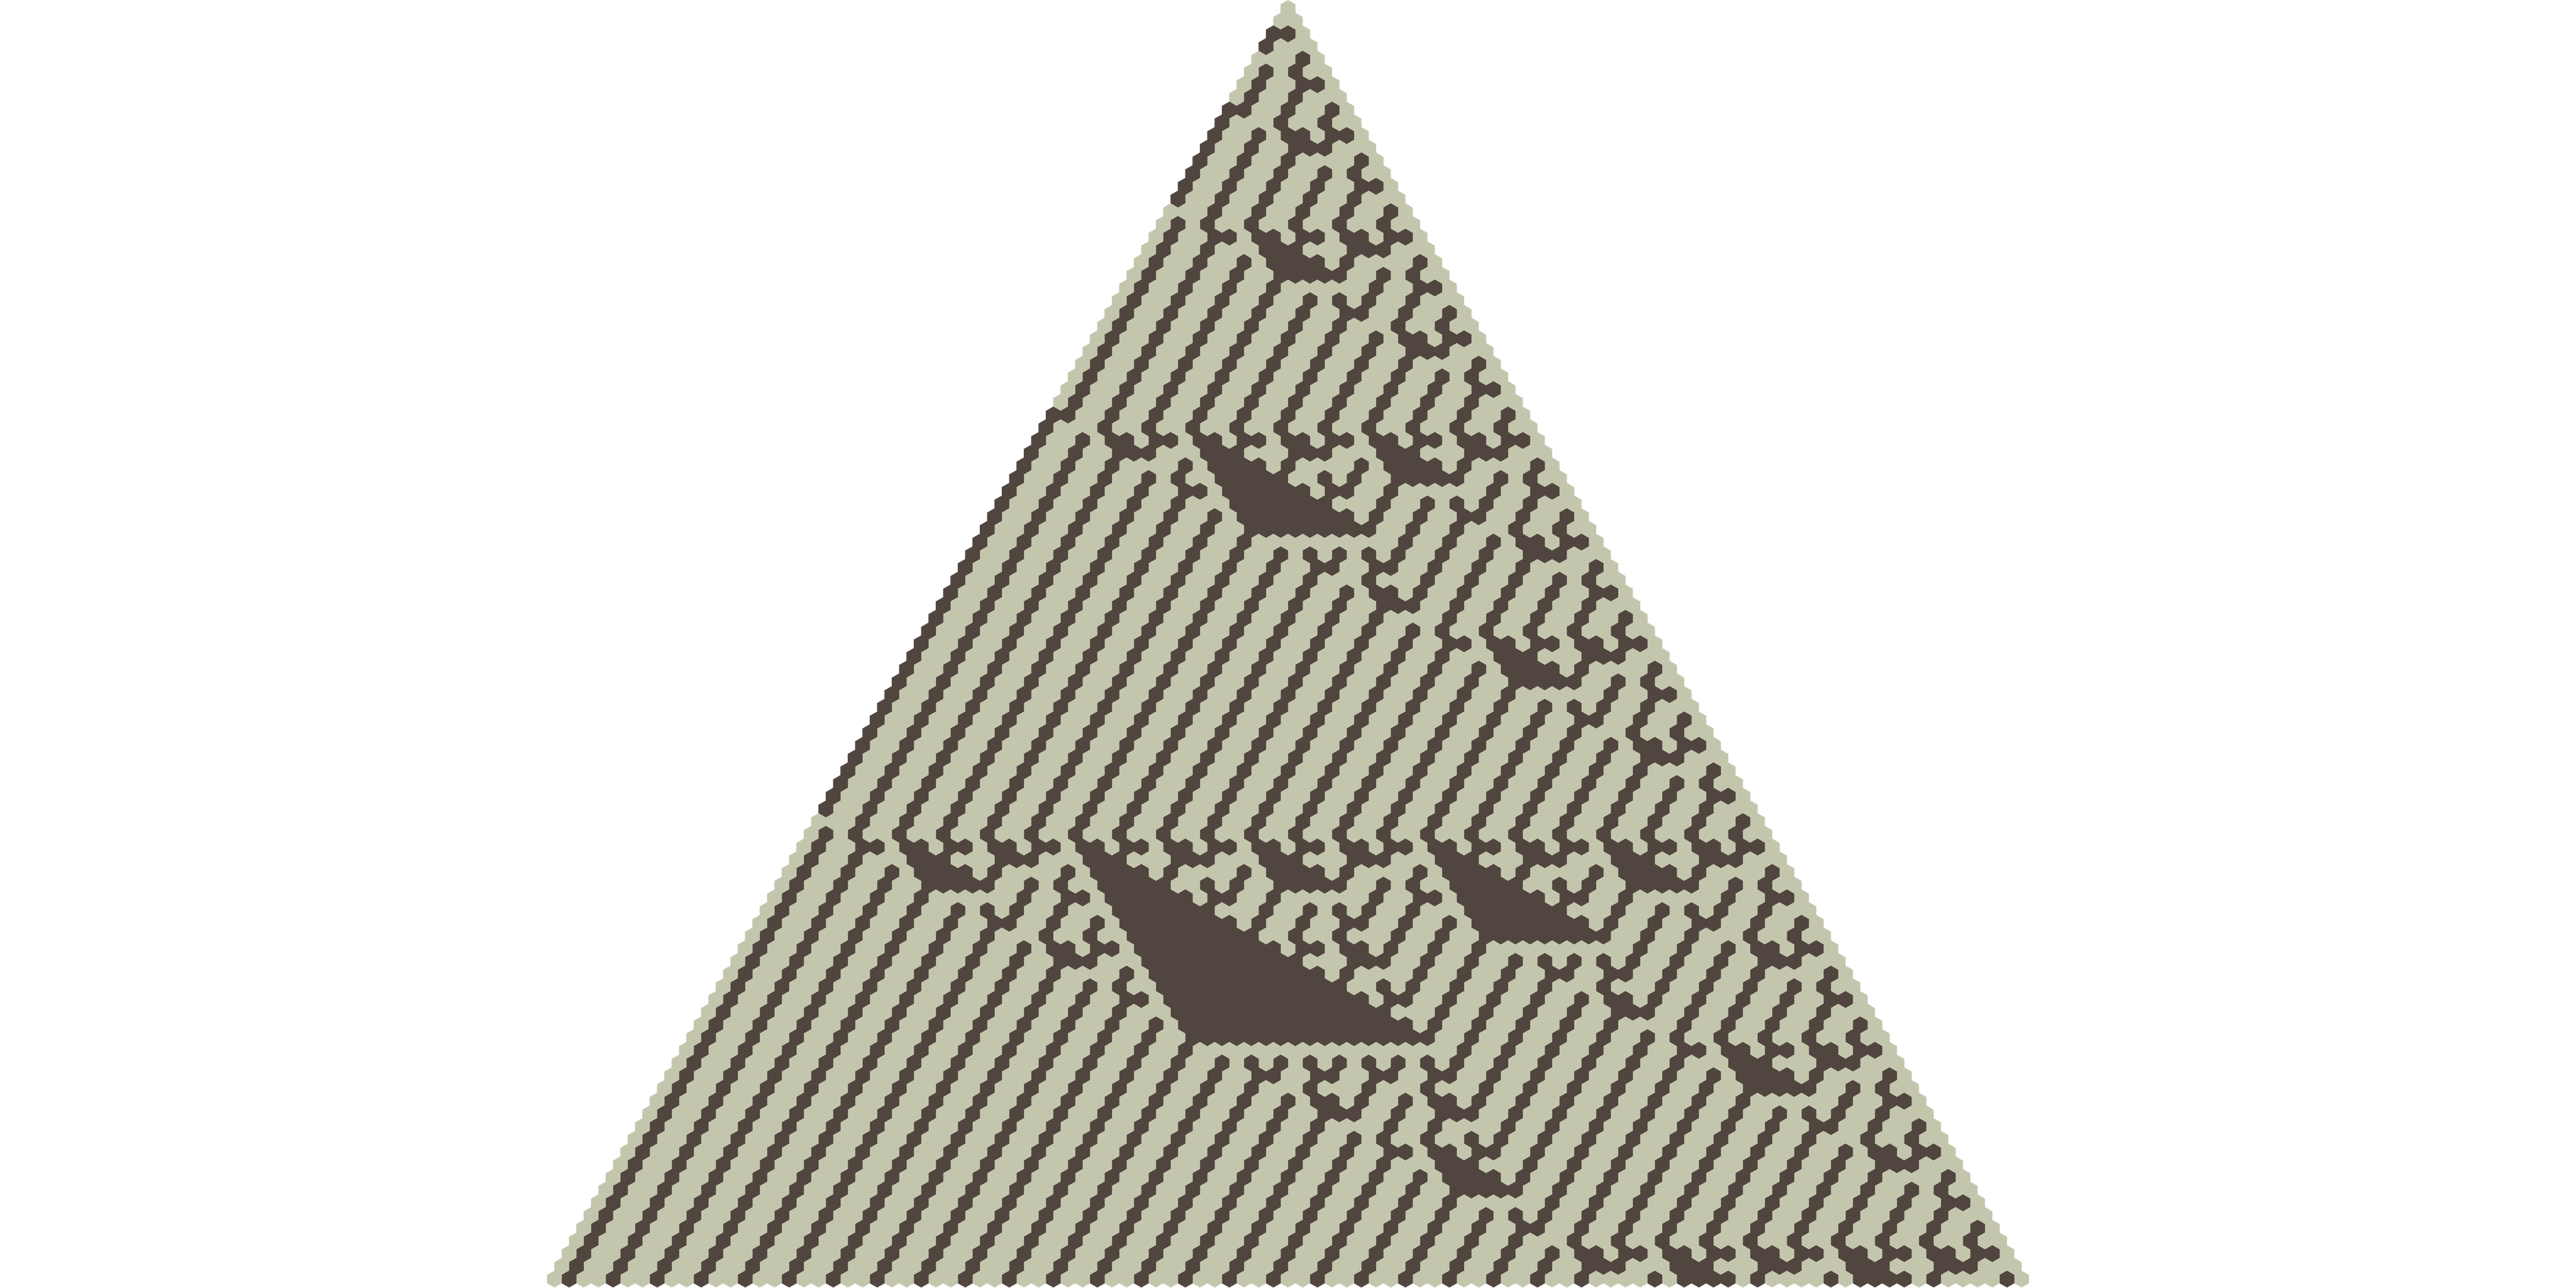
\includegraphics[trim={800 0 800 0}, clip, width=4cm]{assets/128_problem/A236830_2022-11-03.png}
% 
\includegraphics[trim={800 0 800 0}, clip, width=4cm]{assets/128_problem/A238341_2021-11-30.png}
% 
\includegraphics[trim={800 0 800 0}, clip, width=4cm]{assets/128_problem/A242451_2022-07-17.png}
% 
\includegraphics[trim={800 0 800 0}, clip, width=4cm]{assets/128_problem/A247299_2021-04-05.png}
% 
\includegraphics[trim={800 0 800 0}, clip, width=4cm]{assets/128_problem/A258170_2022-06-11.png}
% 
\includegraphics[trim={800 0 800 0}, clip, width=4cm]{assets/128_problem/A273897_2021-08-10.png}
% 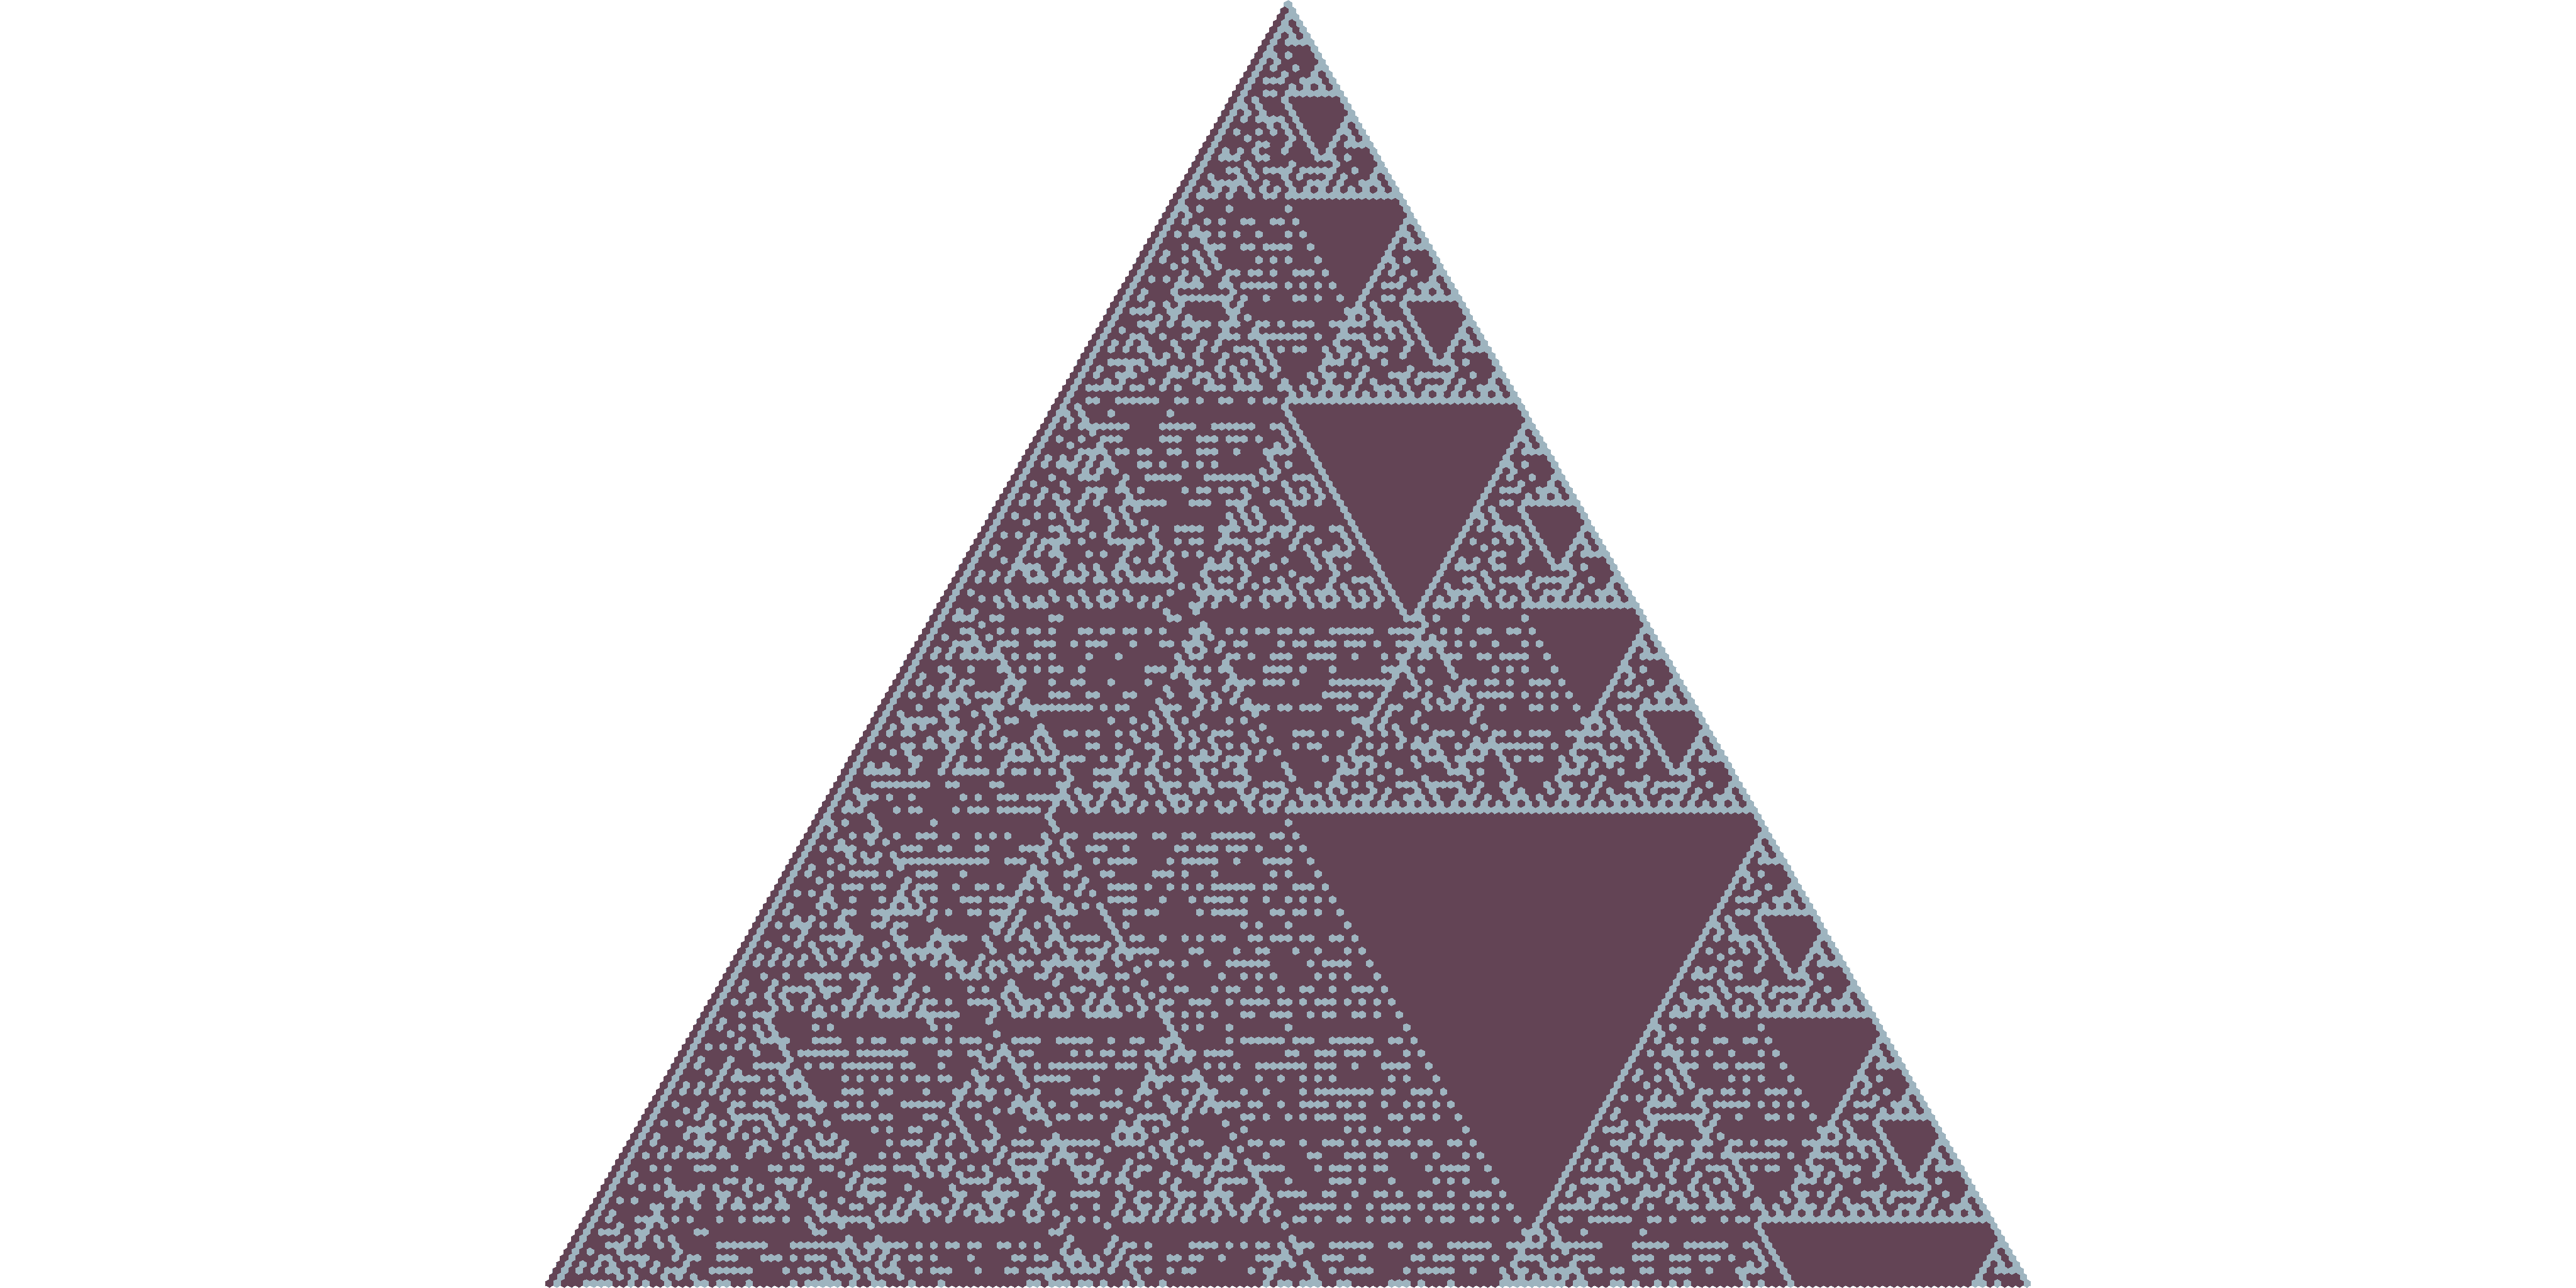
\includegraphics[trim={800 0 800 0}, clip, width=4cm]{assets/128_problem/A275281_2022-02-22.png}
% 
\includegraphics[trim={800 0 800 0}, clip, width=4cm]{assets/128_problem/A286416_2021-08-27.png}
% 
\includegraphics[trim={800 0 800 0}, clip, width=4cm]{assets/128_problem/A297497_2022-05-21.png}
% 
\includegraphics[trim={800 0 800 0}, clip, width=4cm]{assets/128_problem/A309049_2021-11-29.png}
% 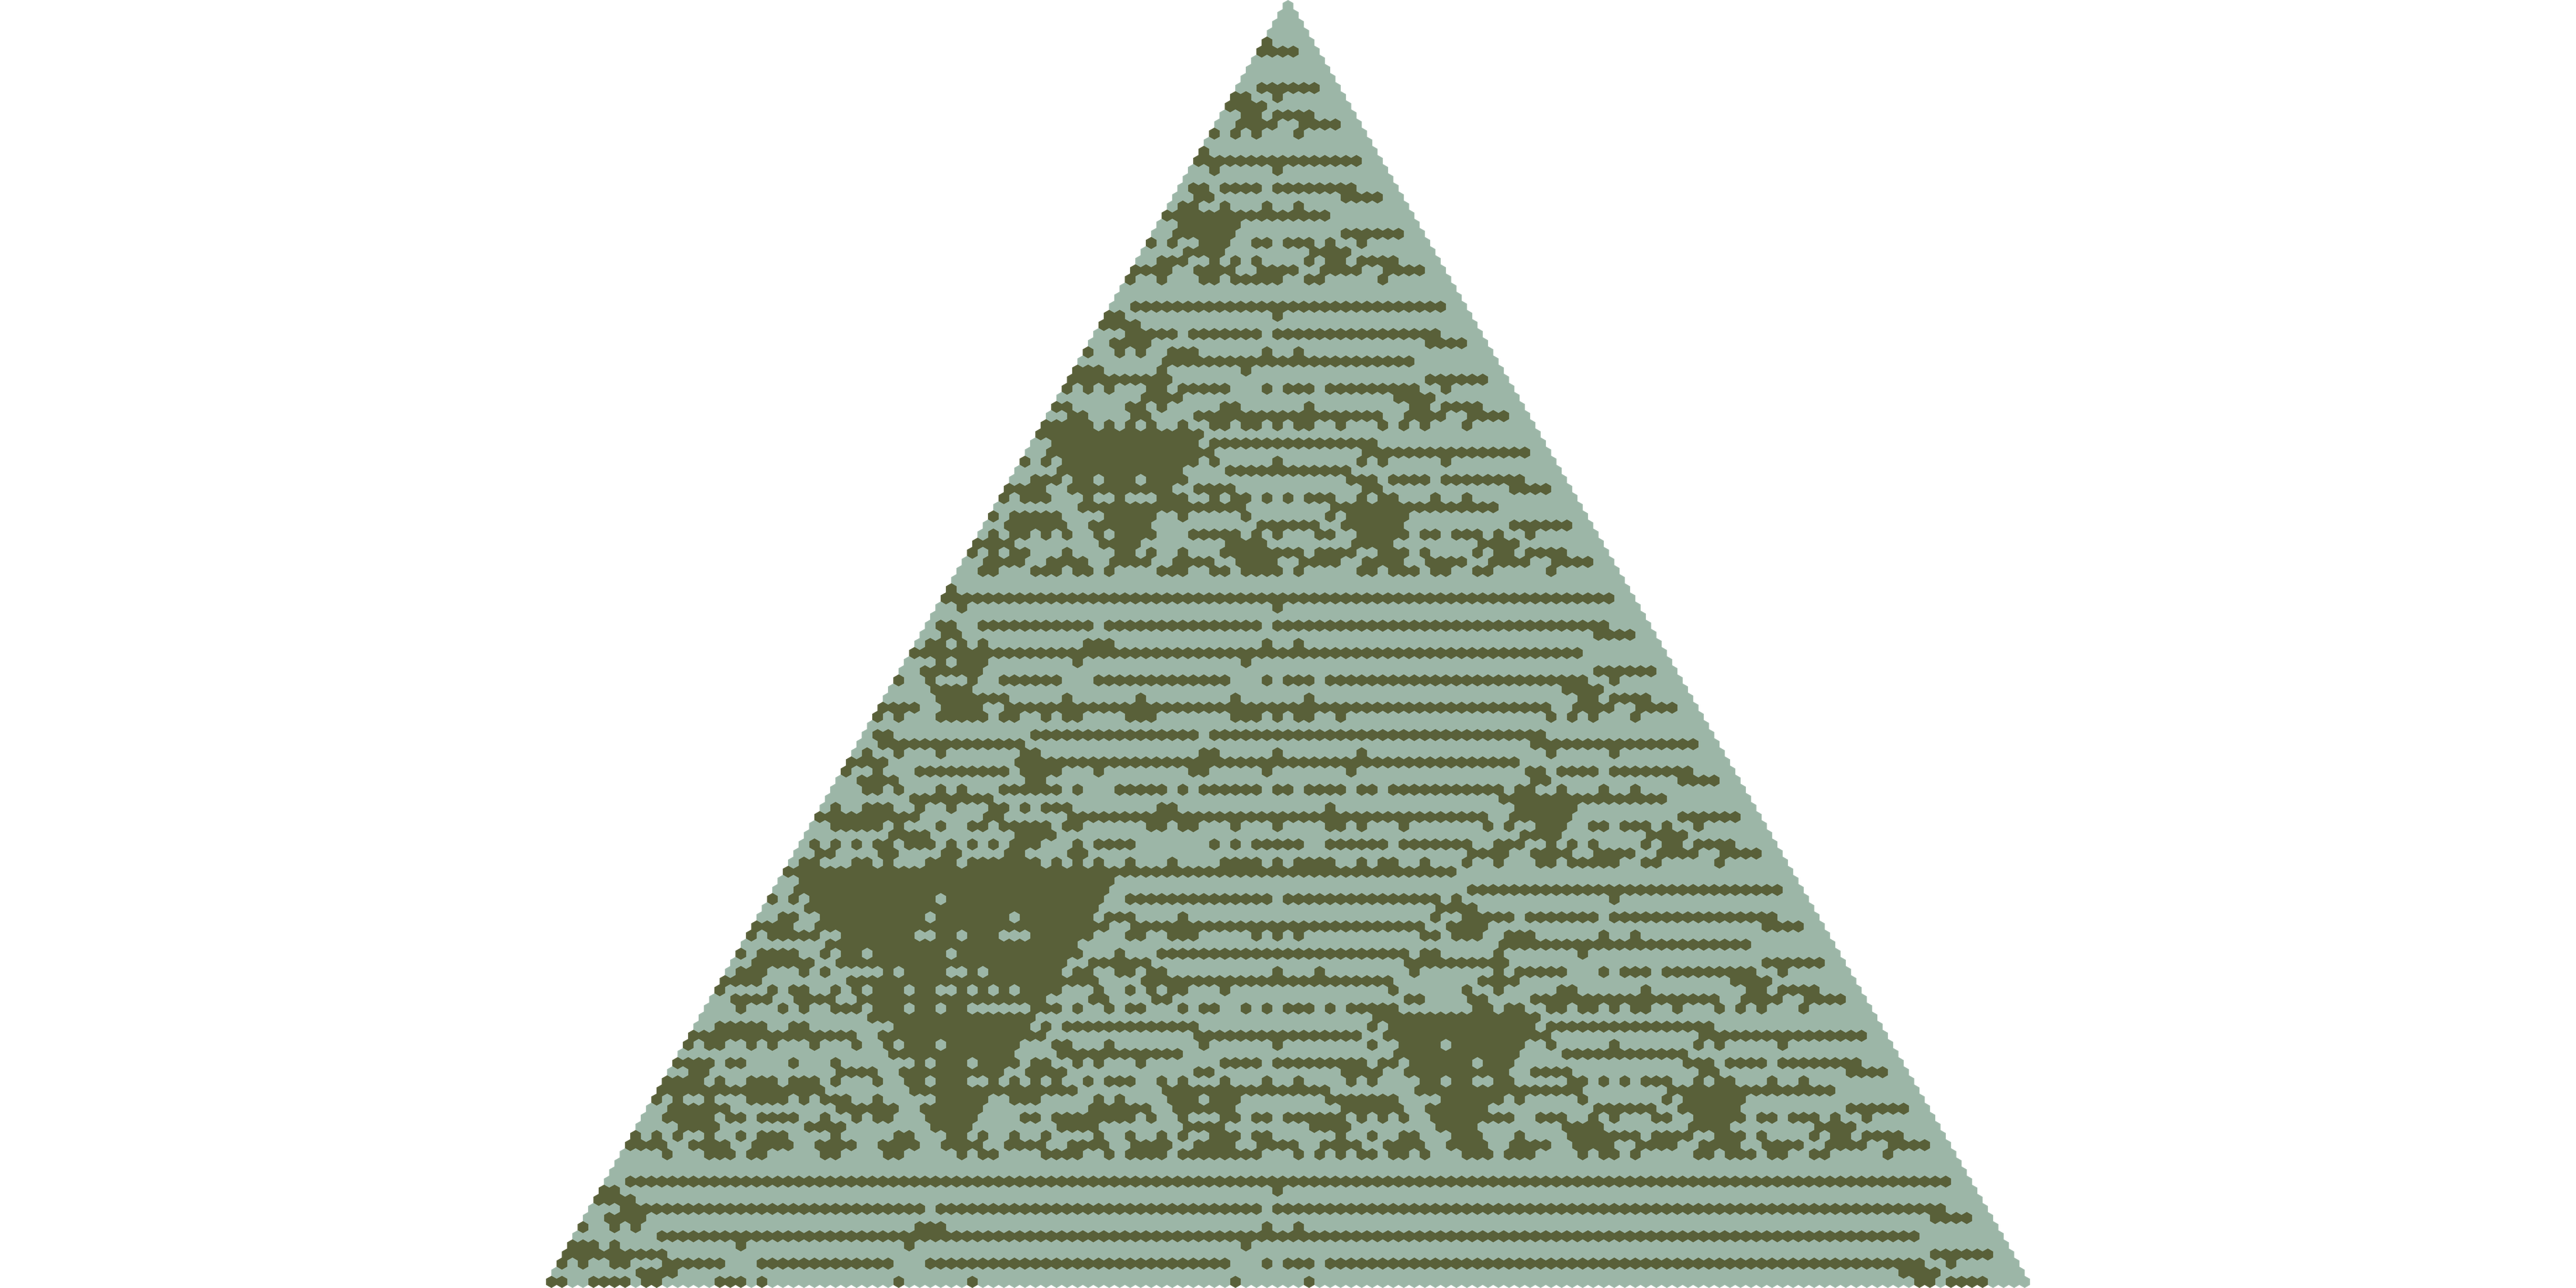
\includegraphics[trim={800 0 800 0}, clip, width=4cm]{assets/128_problem/A319298_2022-12-13.png}
% 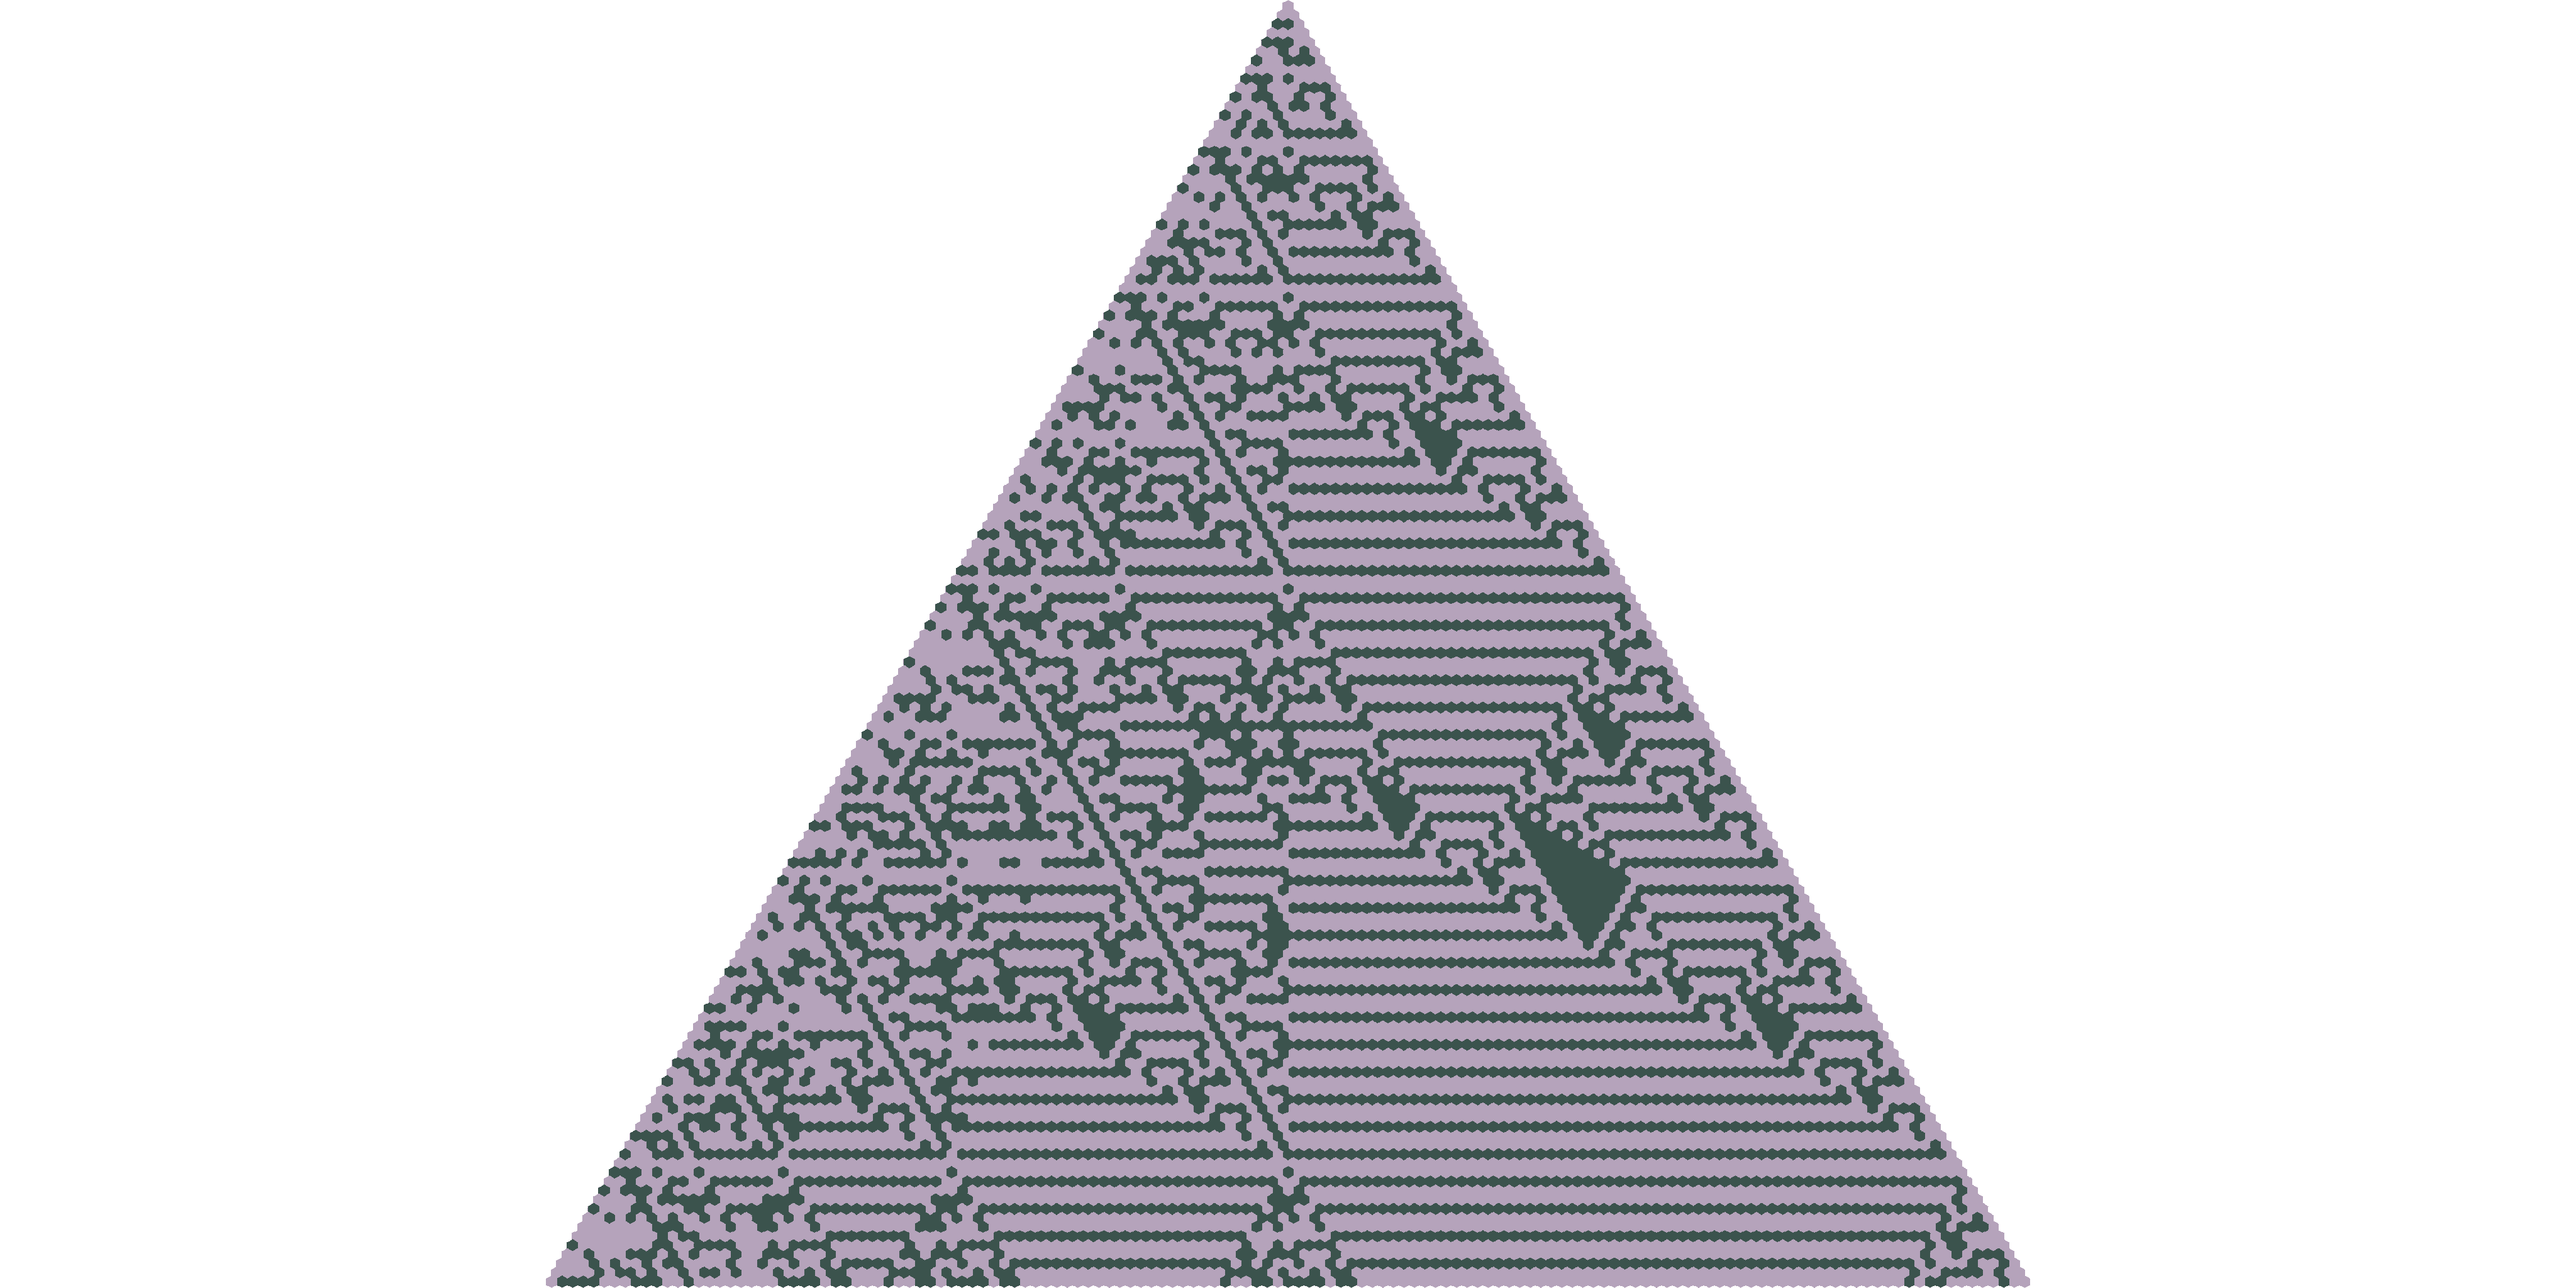
\includegraphics[trim={800 0 800 0}, clip, width=4cm]{assets/128_problem/A319375_2021-04-06.png}
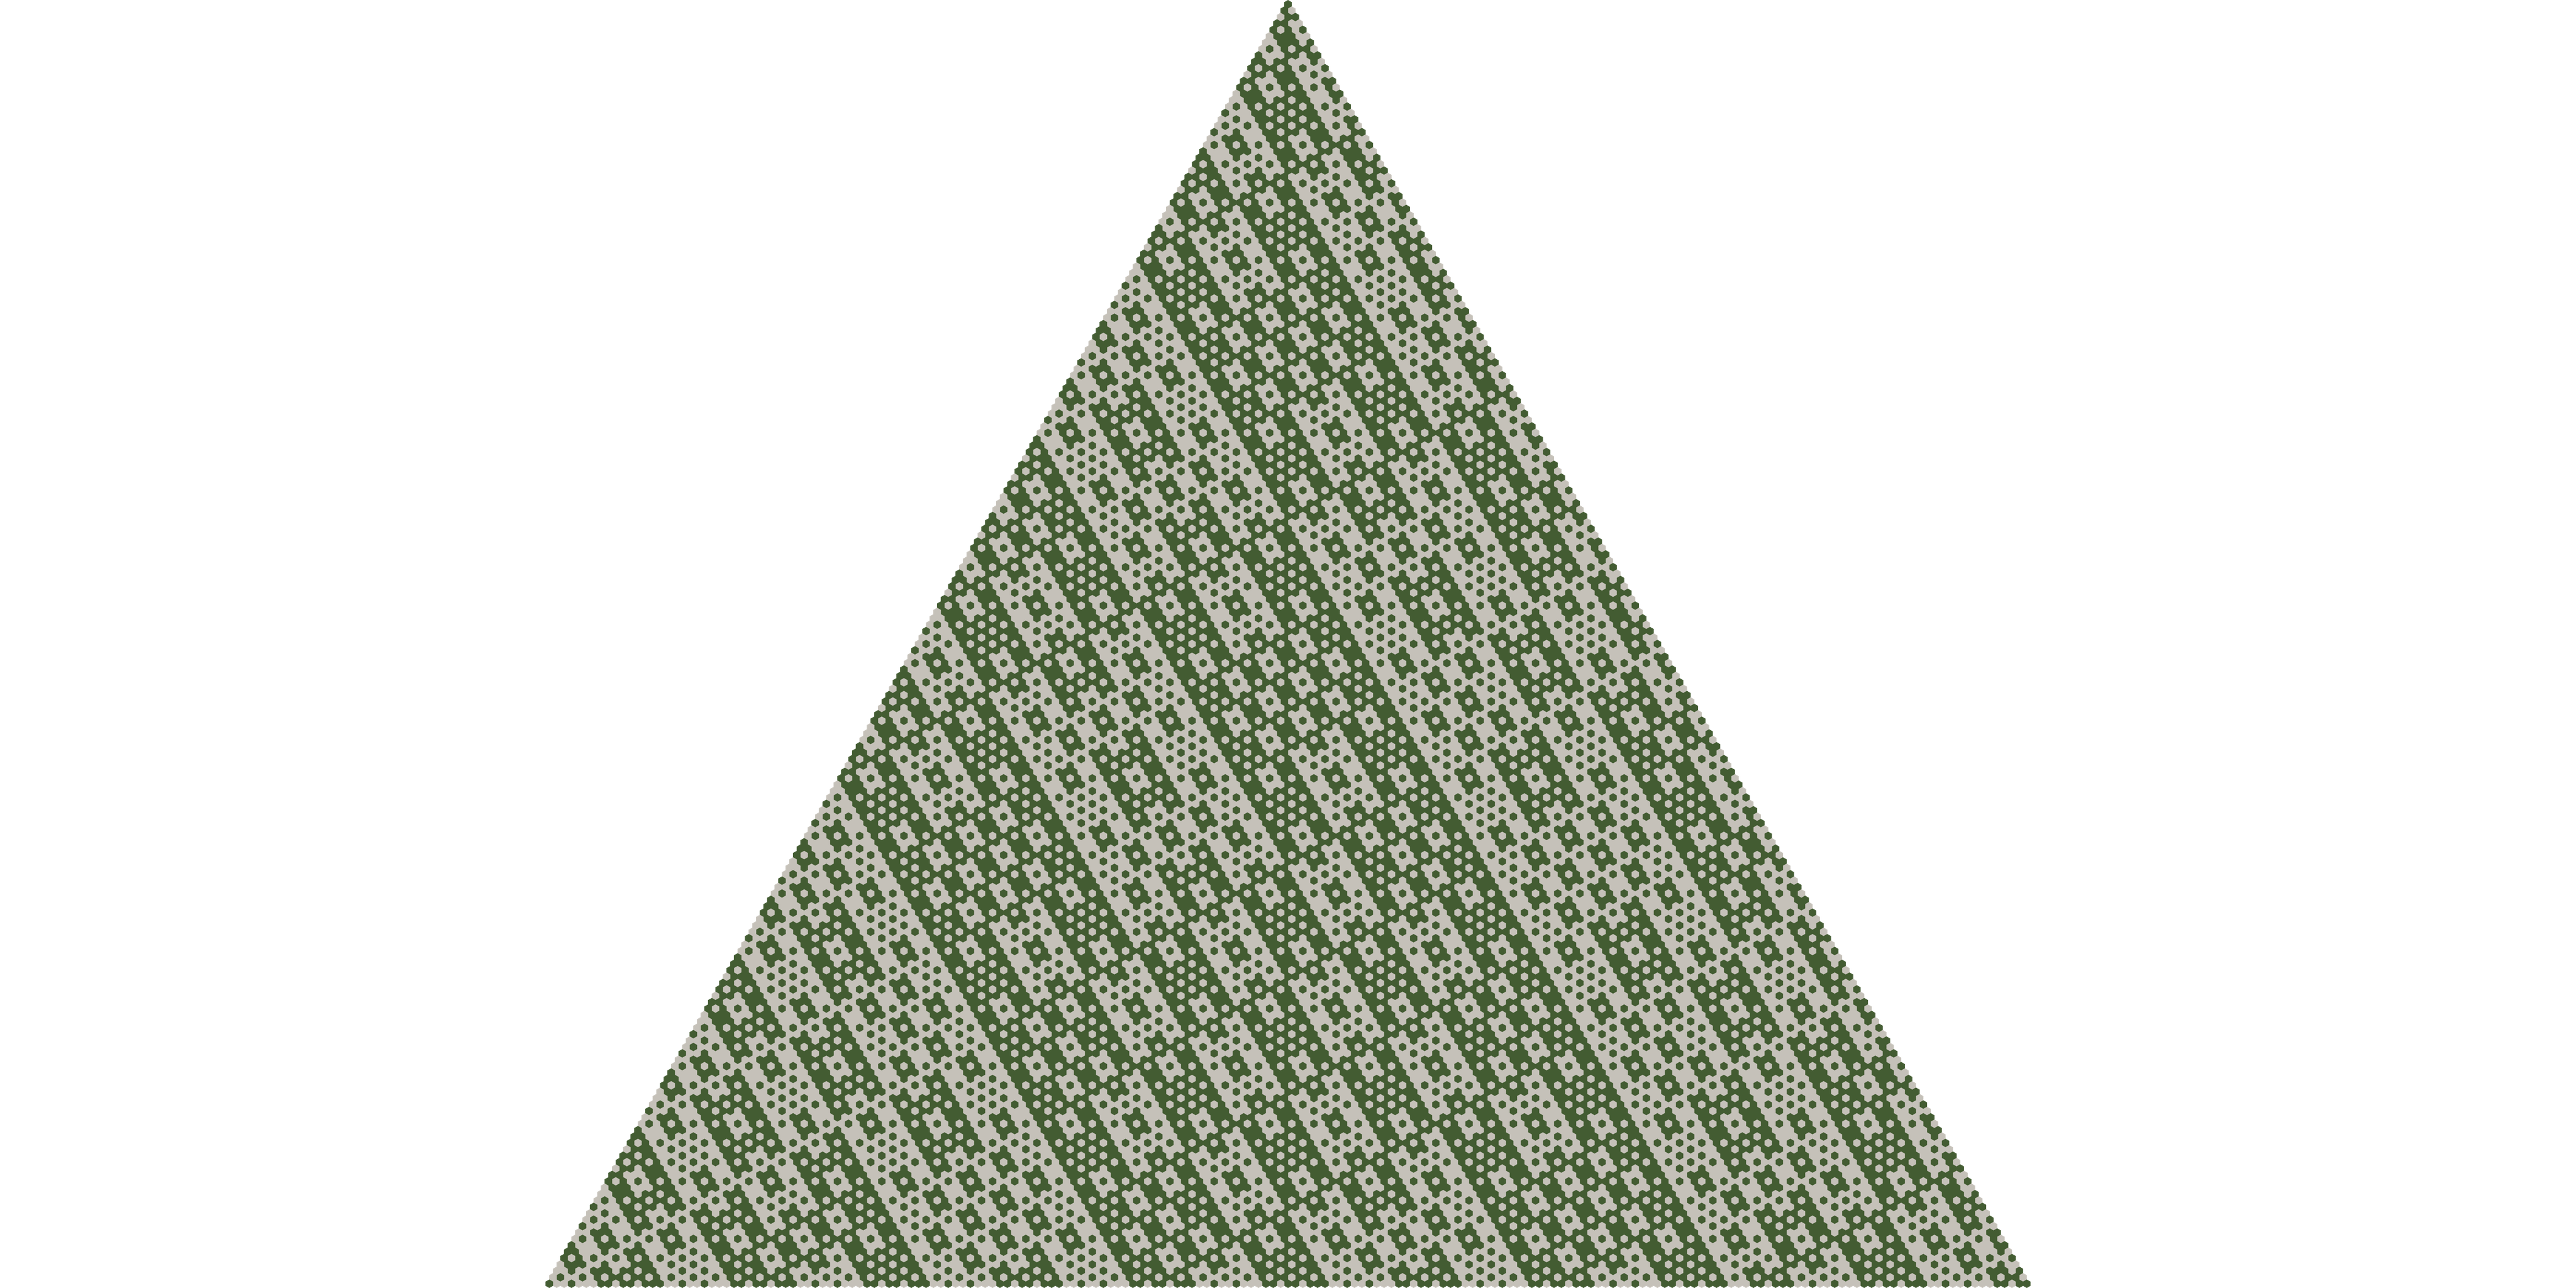
\includegraphics[trim={800 0 800 0}, clip, width=4cm]{assets/128_problem/A253587_2022-12-01.png}

\includegraphics[trim={800 0 800 0}, clip, width=4cm]{assets/128_problem/A273899_2022_11-27.png}
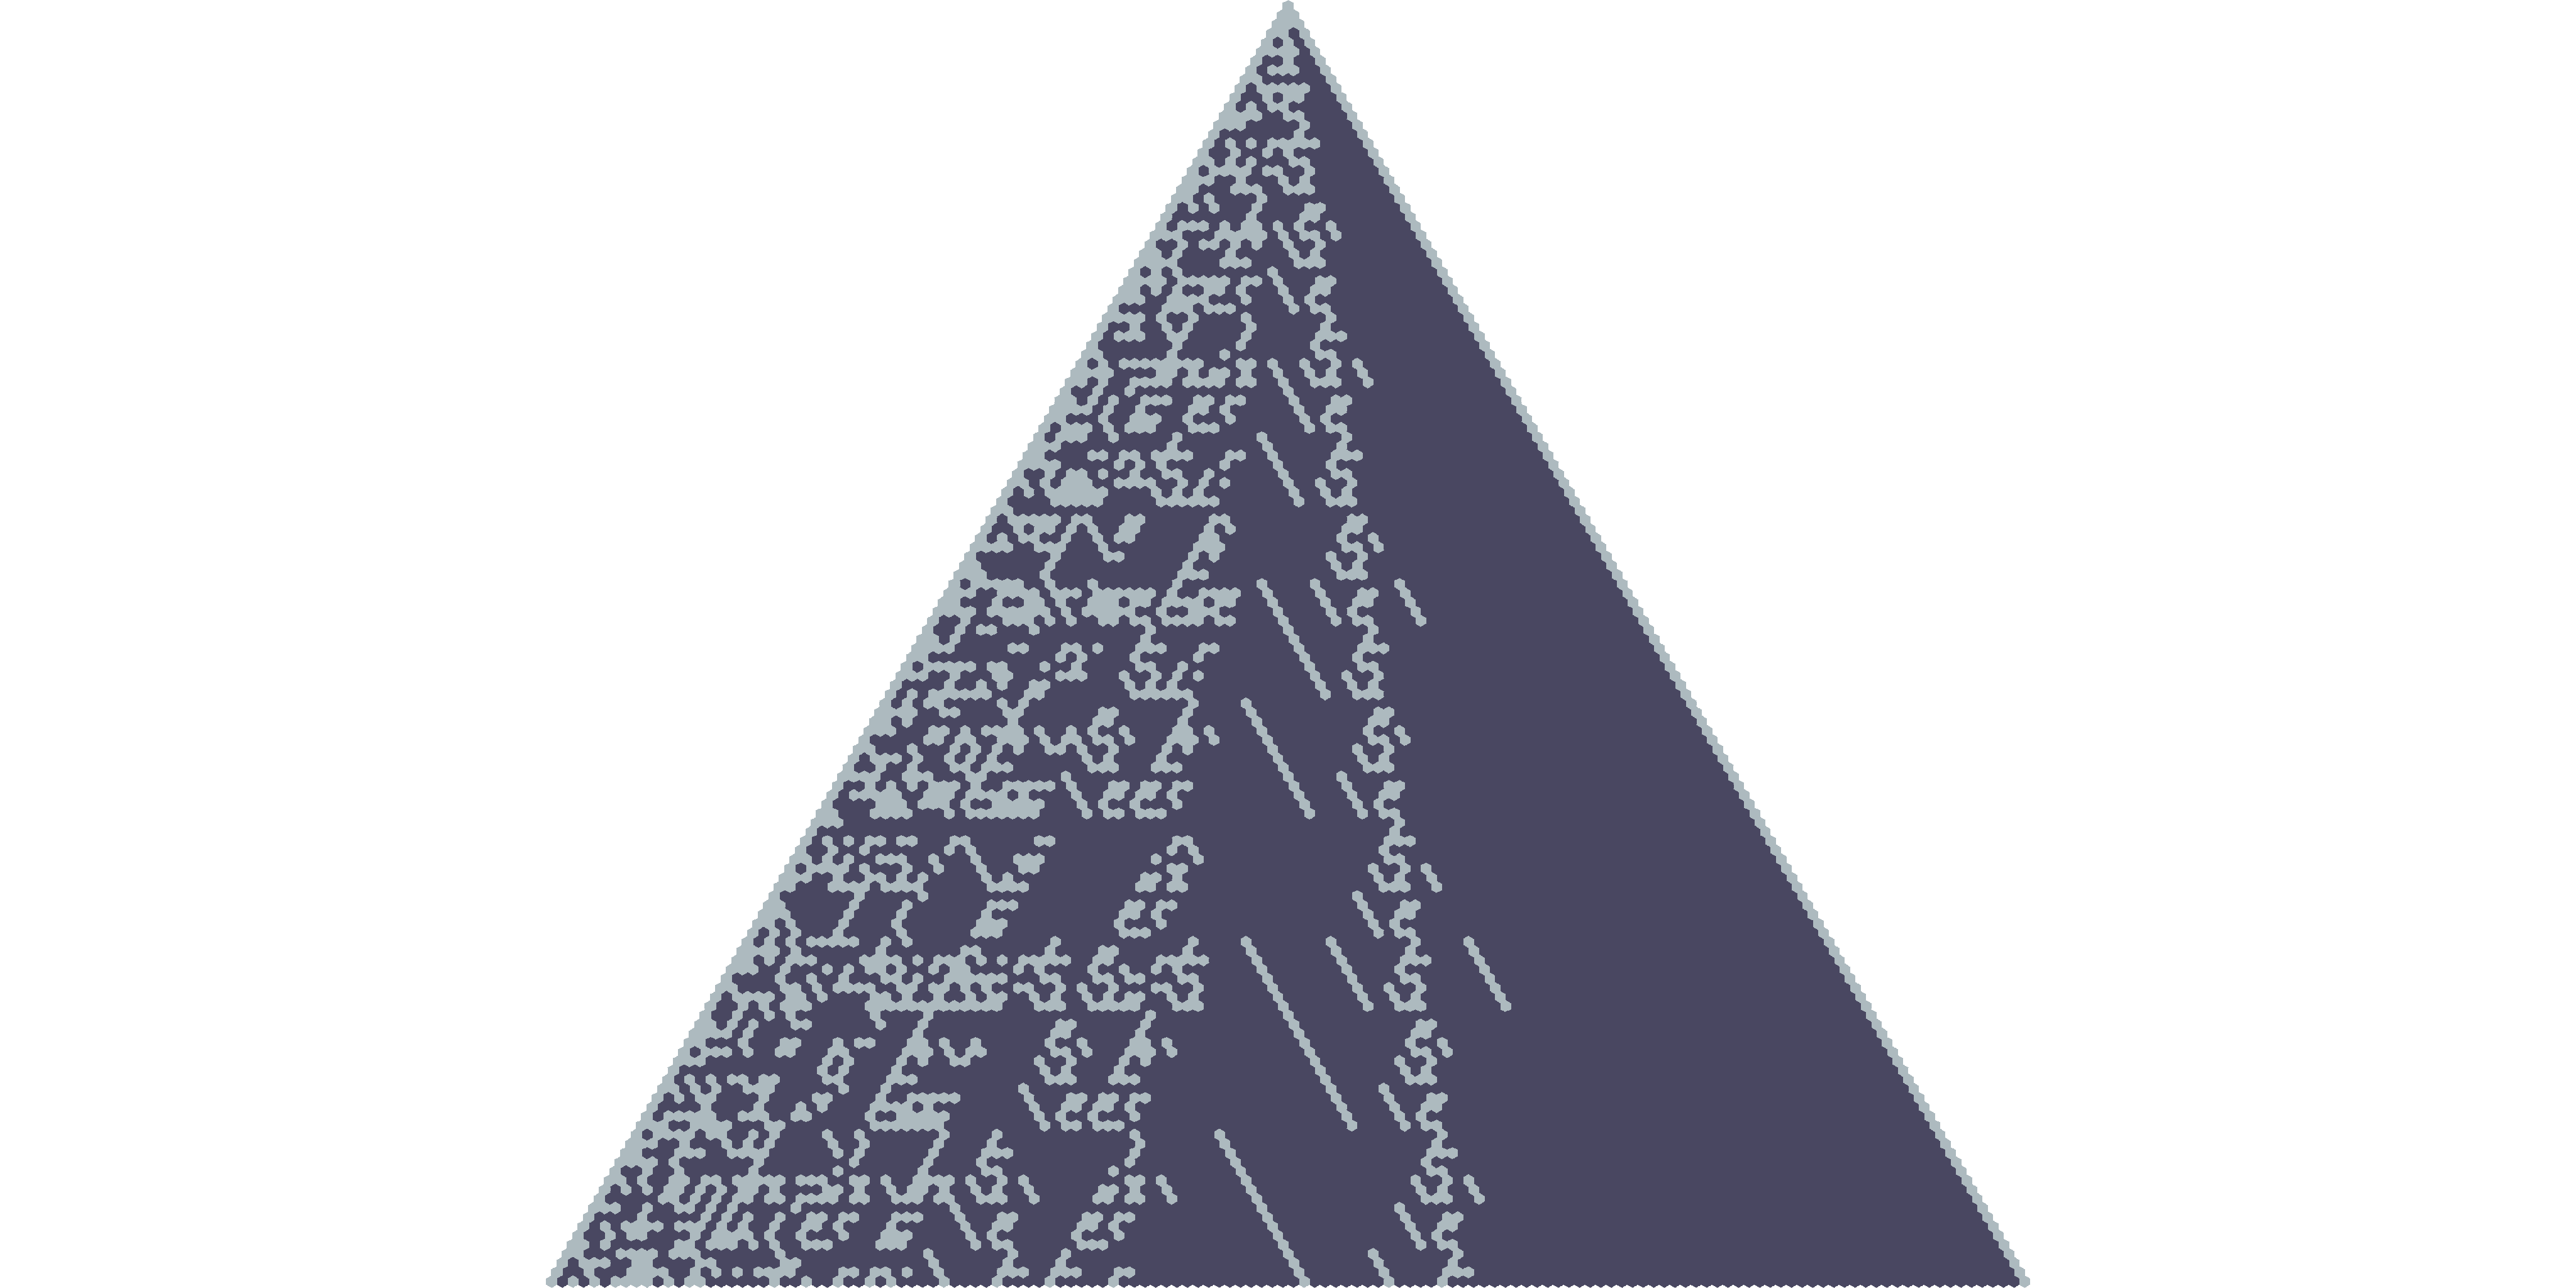
\includegraphics[trim={800 0 800 0}, clip, width=4cm]{assets/128_problem/A282716_2022-09-18.png}
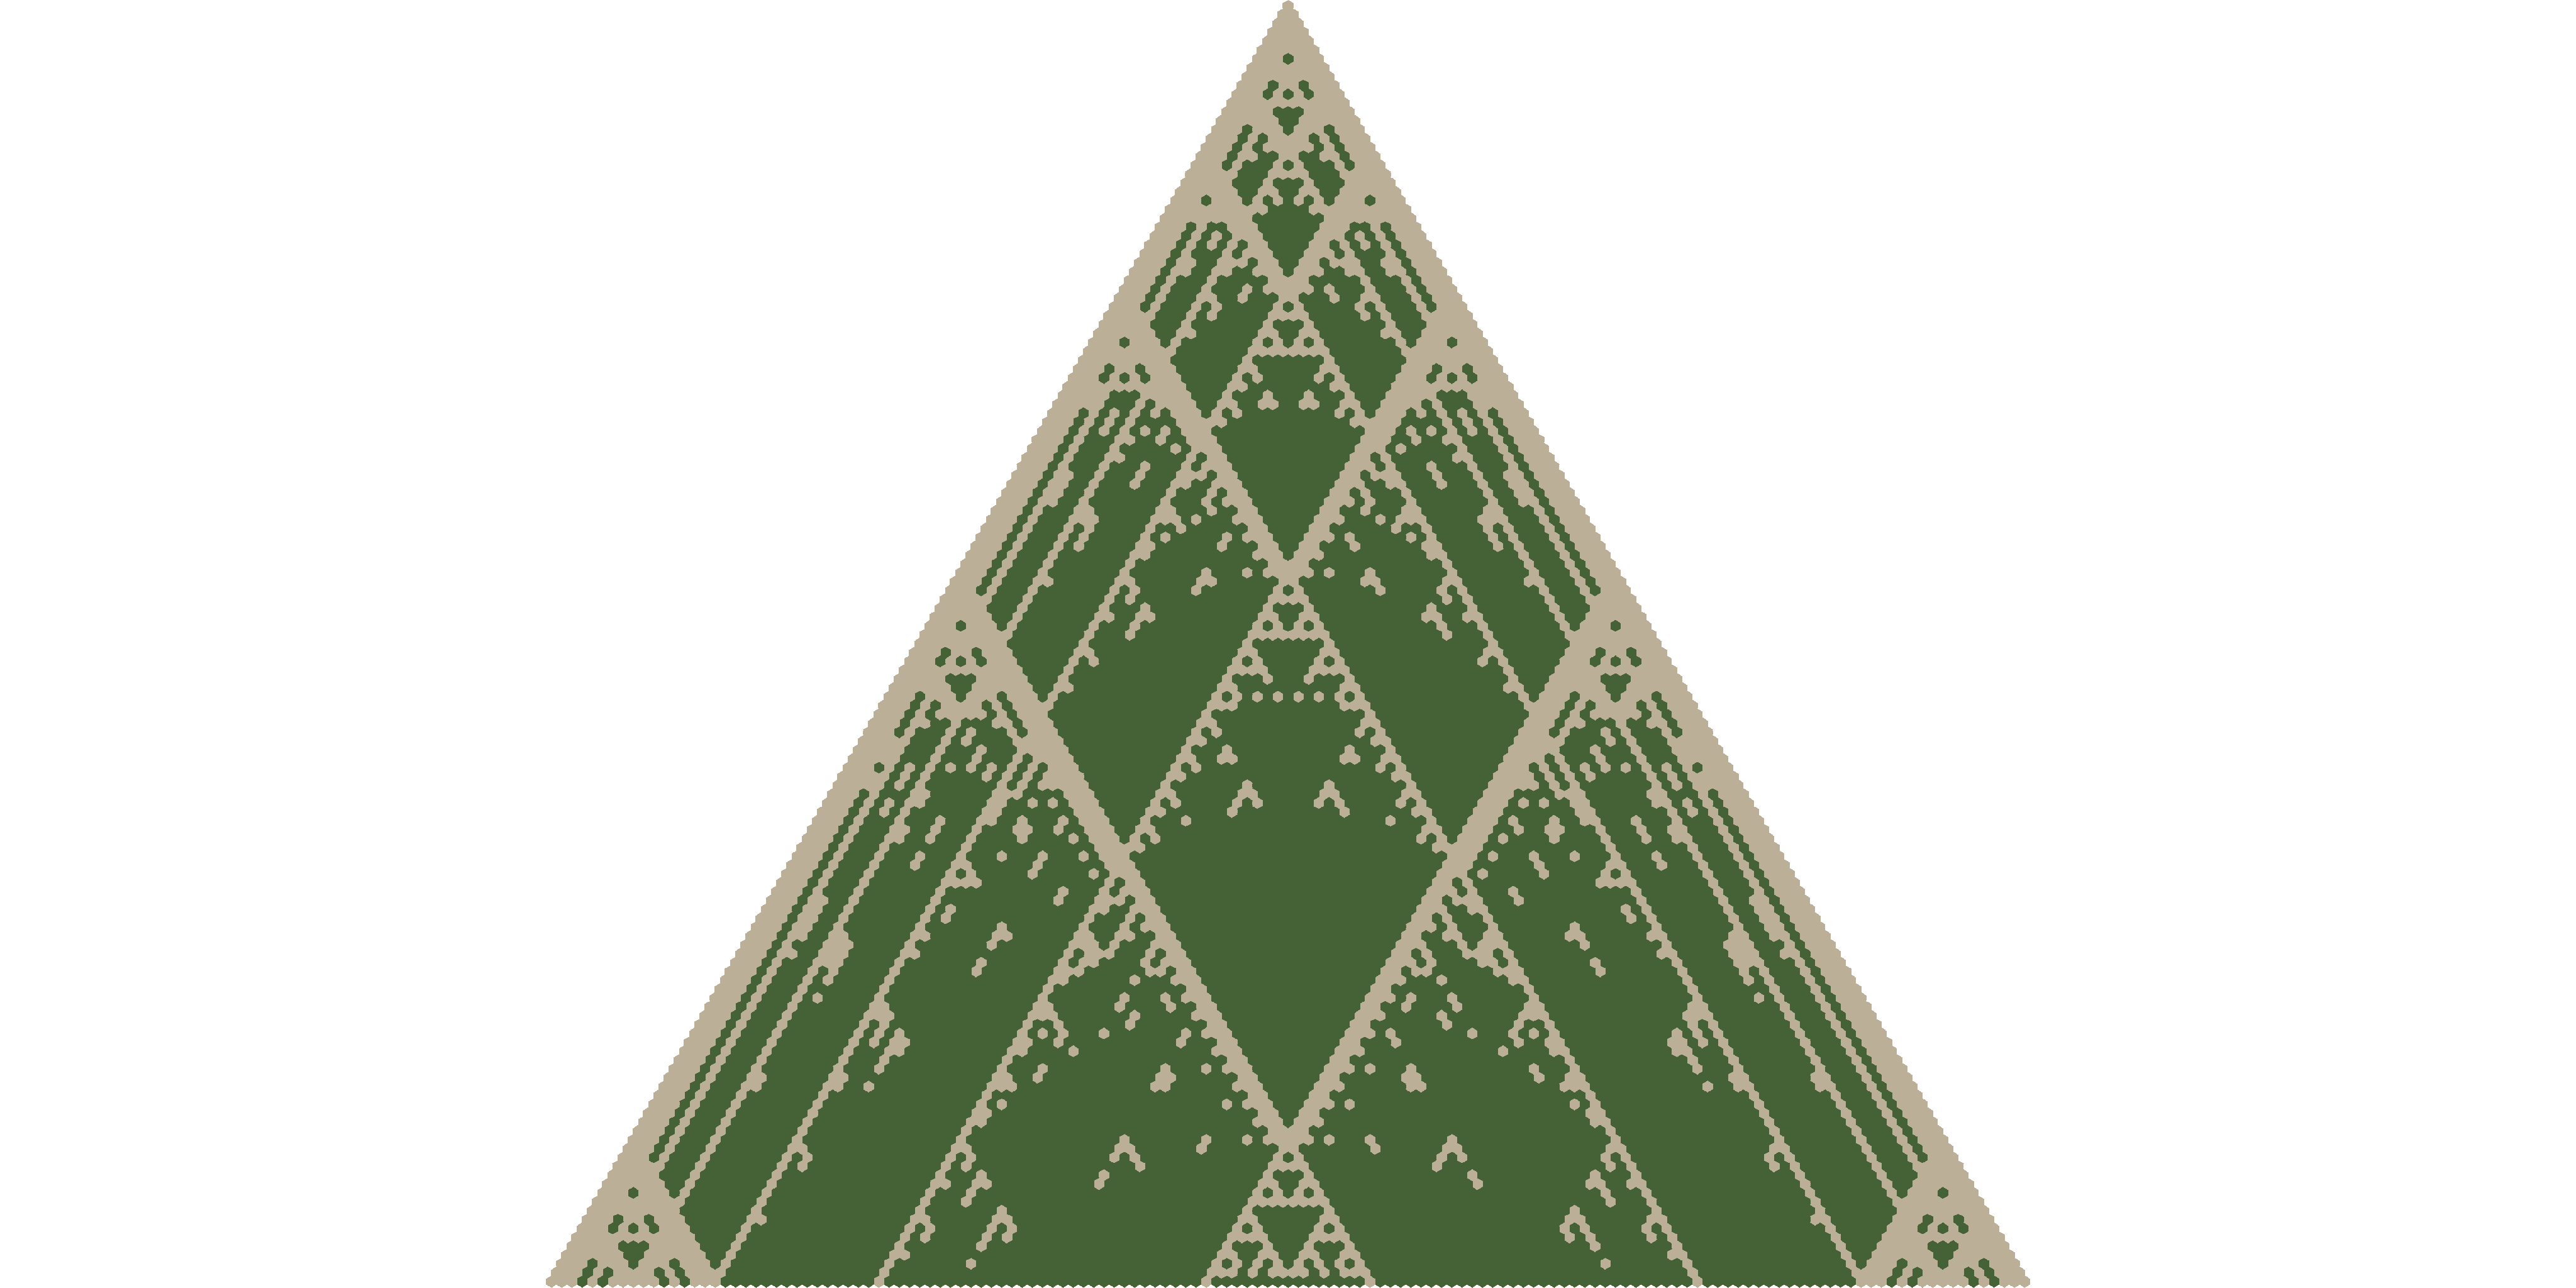
\includegraphics[trim={800 0 800 0}, clip, width=4cm]{assets/128_problem/A322674_2021-10-03.png}
\caption{
  Parity triangles for OEIS sequences A253587, A273899, A282716, and A322674.
}
\end{figure}

\begin{question}
  How can one algorithmically determine the fractal dimension of parity
  triangles given by various families of generating functions, specifically
  those shown in the figures above.
\end{question}

\begin{related}
  \item Does the fractal dimension depend on how many rows are shown?
  (e.g. in Figure 1, we consider the limiting shape for $2^n$ rows, what if we
  considered $3(2^n)$ rows or something like this instead?)
  \item How might this work for other geometries: tetrahedra,
  $n$-simplices, squares, diamonds (i.e. two equilateral triangles together), etc.
\end{related}

\begin{references}
  \item Problem 122.
  \item \href{https://math.stackexchange.com/q/4554568/121988}{Peter Kagey, Math Stack Exchange}.
  \item Twitter bot, \href{https://twitter.com/oeisTriangles}{@oeisTriangles}.
  \item Peter Kagey's blog, \href{https://blog.peterkagey.com/2021/03/parity-bitmaps-from-the-oeis/}{Parity Bitmaps from the OEIS}.
\end{references}
\end{document}

